\documentclass[final]{beamer}
%% Possible paper sizes: a0, a0b, a1, a2, a3, a4.
%% Possible orientations: portrait, landscape
%% Font sizes can be changed using the scale option.
\usepackage[size=a3,orientation=portrait,scale=1.1]{beamerposter}

\usetheme{gemini}
\usecolortheme{seagull}
\useinnertheme{rectangles}

% ====================
% Packages
% ====================

\usepackage[utf8]{inputenc}
\usepackage{graphicx}
\usepackage{booktabs}
\usepackage{tikz}
\usepackage{pgfplots}

% ====================
% Lengths
% ====================

% If you have N columns, choose \sepwidth and \colwidth such that
% (N+1)*\sepwidth + N*\colwidth = \paperwidth
\newlength{\sepwidth}
\newlength{\colwidth}
\setlength{\sepwidth}{0.03\paperwidth}
\setlength{\colwidth}{0.45\paperwidth}

\newcommand{\separatorcolumn}{\begin{column}{\sepwidth}\end{column}}

% ====================
% Logo (optional)
% ====================

% LaTeX logo taken from https://commons.wikimedia.org/wiki/File:LaTeX_logo.svg
% use this to include logos on the left and/or right side of the header:
%\logoright{\includegraphics[height=5cm]{logos/1200px-LaTeX_logo.svg.png}}
%\logoleft{\includegraphics[height=5cm]{logos/1200px-LaTeX_logo.svg.png}}

% ====================
% Footer (optional)
% ====================

\footercontent{
	T-424 SLEE \hfill
	March 4, 2026 \hfill
	{\href{nils25@ru.is}{\texttt{nils25@ru.is}}, 
    \href{martin25@ru.is}{\texttt{martin25@ru.is}}}
}
% (can be left out to remove footer)

% ====================
% My own customization
% - BibLaTeX
% - Boxes with tcolorbox
% - User-defined commands
% ====================
\input{custom-defs.tex}

%% Reference Sources
\addbibresource{refs.bib}
\renewcommand{\pgfuseimage}[1]{\includegraphics[scale=2.0]{#1}}

\title{Sleep Stage Scoring with Polysomnography (PSG)}

\author{Nils Wagner \inst{1} \and Martin Gaens \inst{1}}

\institute[shortinst]{\inst{1} Reykjavik University} % \samelineand \inst{2} Another Institute}

%\date{January 01, 2025}


\newcommand{\tbd}[1]{{\color{red} TBD #1}}

\begin{document}
	
\begin{frame}[t]
	
	\begin{columns}[t]
	
	\begin{column}{2\colwidth+\sepwidth}
	\begin{block}{Introduction to Sleep Stages}
        \begin{columns}[t]
            \begin{column}{\colwidth}
                \vspace{-0.8cm}
                \begin{figure}
    			\centering
    			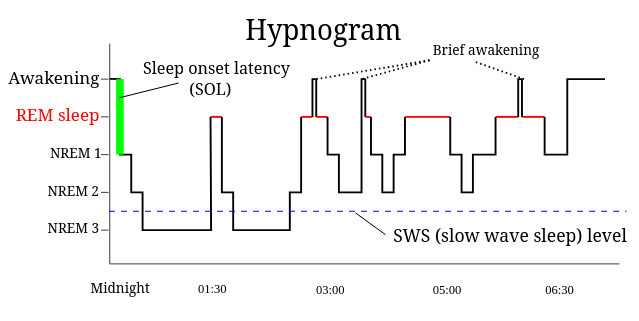
\includegraphics[width=12cm]{imgs/hypnogram.png}
    			\caption{Hypnogram of healthy adult}
    		\end{figure}
            \end{column}
            \begin{column}{\colwidth}
                \vspace{-0.3cm}
                \begin{itemize}
                    \item Sleep is a biological process essential for brain function, cardiovascular health, immune regulation, and emotional stability
                    \item Two main types: \textbf{Non-REM sleep} (stages N1, N2, N3) and \textbf{REM sleep}
                    \item Each stage has distinct physiological characteristics measurable through EEG, EOG, and EMG
                \end{itemize}
                \heading{Sleep Stage Characteristics and Functions}
                \begin{itemize}
                    \item \textbf{REM (Dream Sleep)}: $20-25\%$ of total sleep; essential for emotional regulation and procedural memory consolidation
                    \item \textbf{N1 (Light Transitional)}: $<5\%$ of total sleep; transition between wakefulness and sleep
                    \item \textbf{N2 (Stable Light Sleep)}: largest proportion of total sleep; supports sensory processing and memory consolidation
                    \item \textbf{N3 (Deep Sleep)}: critical for physical restoration, immune function, and declarative memory consolidation; reduced with aging
                \end{itemize}
            \end{column}
        \end{columns}
	\end{block}
	\end{column}

	\end{columns}

	\begin{columns}[t]
		\separatorcolumn
		
		\begin{column}{\colwidth}

            \begin{block}{Sleep Scoring}
                \begin{itemize}
                    \item According to guidelines in American Academy of Sleep Medicine (AASM) manual
                    \item Recording divided into \textbf{30-second epochs}, each classified by \textbf{sleep stage} based on EEG, EOG and EMG signals
                    \item \textbf{Respiratory events} (apneas, hypopneas) scored according to airflow, effort and oxygen desaturation criteria
                    \item Arousals, movement-related events, and snoring also annotated
                \end{itemize}


            \heading{Signals from Frontal EEG in Self-applied PSG \cite{nox_sas_signals_impedance_2024}}
            
            \begin{columns}[t]
            
                 \begin{column}{0.5\colwidth}
                 \vspace{-0.5cm}
                    \begin{figure}
                        \centering
                        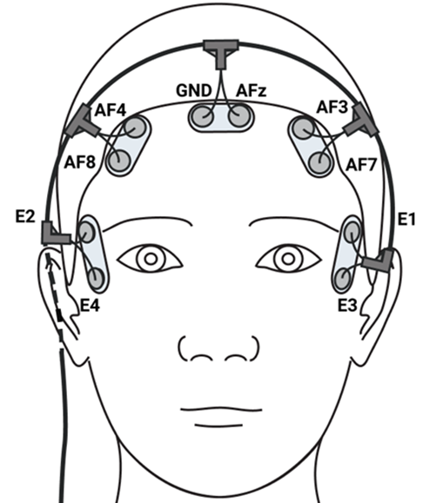
\includegraphics[width=0.6\linewidth]{imgs/frontal_psg2.png}
                        \caption{Placement of electrodes in self-applied PSG}
                        \label{fig:electrodesPSG}
                    \end{figure}
                    \vspace{-0.5cm}
                    \begin{itemize}
                        \item \textit{Eye movement (EOG)}: referenced against AFz and cross referenced
                        \item \textit{Brain activity (EEG)}: referenced against average of E3 and E4
                        \item \textit{Muscle tone (EMG)}: EMG temporalis derived from E2-E4 (left) and E1-E3 (right) signal
                        \item No dedicated chin EMG (like in Type 1 PSG)
                    \end{itemize}
                \end{column}
                
                \hspace{-1cm}
                
                \begin{column}{0.4\colwidth}
                \vspace{-0.5cm}
                    \begin{figure}
                        \centering
                        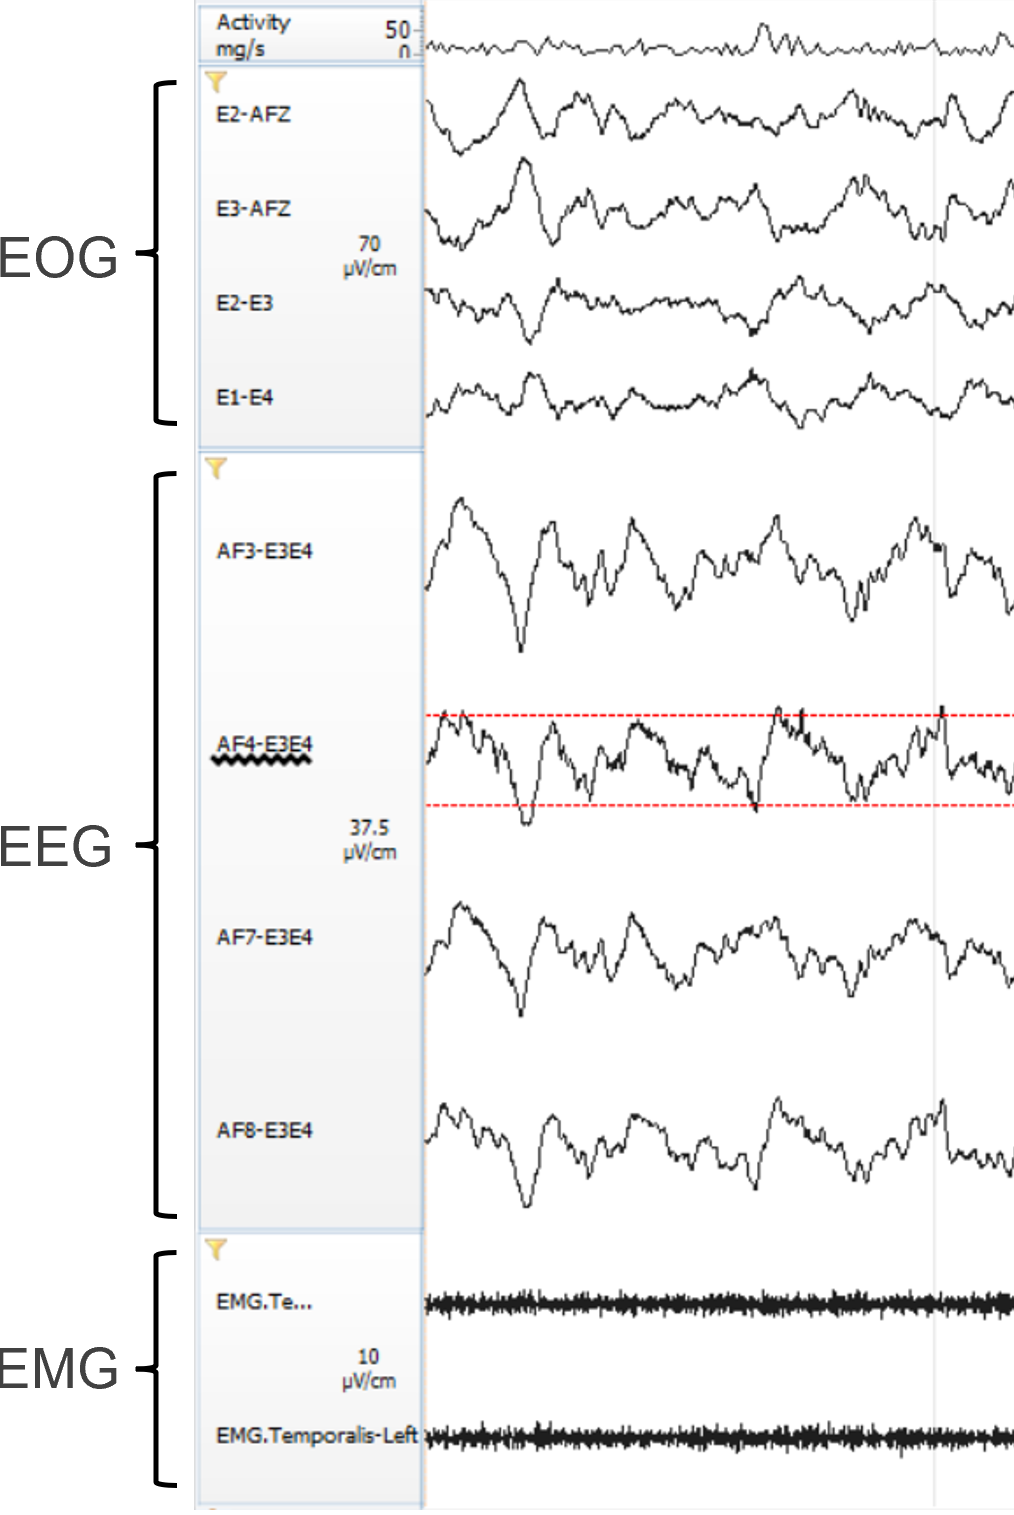
\includegraphics[width=\linewidth]{imgs/annotations.png}
                        \caption{Channels for sleep stage scoring}
                        \label{fig:channels}
                    \end{figure}
                \end{column}
                
            \end{columns}


            \heading{Characteristics of sleep stages}

            \begin{columns}[t]
                \begin{column}{0.65\colwidth}
                    \begin{figure}
                        \centering
                        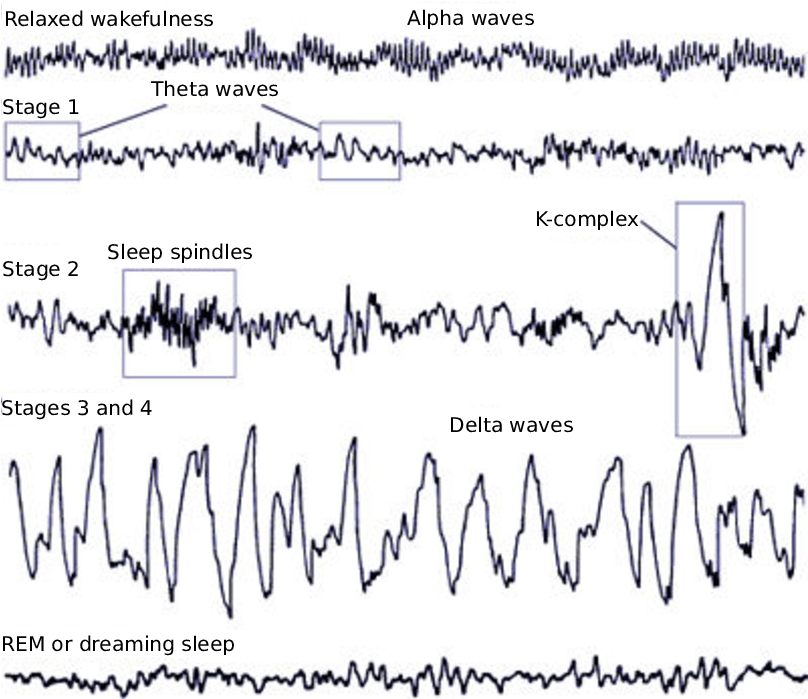
\includegraphics[width=0.92\linewidth]{imgs/characteristics_brain_activity.png}
                        \caption{Characteristic brain wave patterns in different sleep stages \cite{Hitziger2015}}
                        \label{fig:characteristics}
                    \end{figure}
                \end{column}

                \hspace{-1.5cm}
                
                \begin{column}{0.35\colwidth}
                    \begin{itemize}
                        \item \textbf{Wake}: alpha and beta waves, high muscle tone
                        \item \textbf{REM}: rapid eye movements, muscle atonia (lowest muscle tone)
                        \item \textbf{N1}: theta waves, low amplitude and high frequency, brief transitional stage
                        \item \textbf{N2}: sleep spindles and K-complexes, stable light sleep
                        \item \textbf{N3}: high-amplitude, low-frequency synchronized waves, deep restorative sleep
                    \end{itemize}
                \end{column}
            \end{columns}  
            Beta waves ($>$13 Hz), alpha waves (8-13 Hz), theta waves (4-7 Hz), and delta waves ($<$4 Hz) are distinguished by their frequency
            
            \end{block}	
		\end{column}
	
		\separatorcolumn
		
		\begin{column}{\colwidth}
			
            
            \begin{block}{Polysomnography (PSG)}
            
                \begin{itemize}
                    \item Sleep recording/research tool measuring multiple biosignals during sleep
                    \item Records brain activity (EEG), eye movements (EOG), muscle tone (EMG), and respiratory parameters
                    \item Gold standard method for evaluating sleep and sleep disorders
                    \item Used in clinical practice and sleep research
                    \item Types: traditional in-lab PSG (Type 1), self-applied PSG at home (Type 2)
                \end{itemize}
            
                \heading{Set-up of self-applied polysomnography}
                \begin{figure}[h]
                    \centering
                    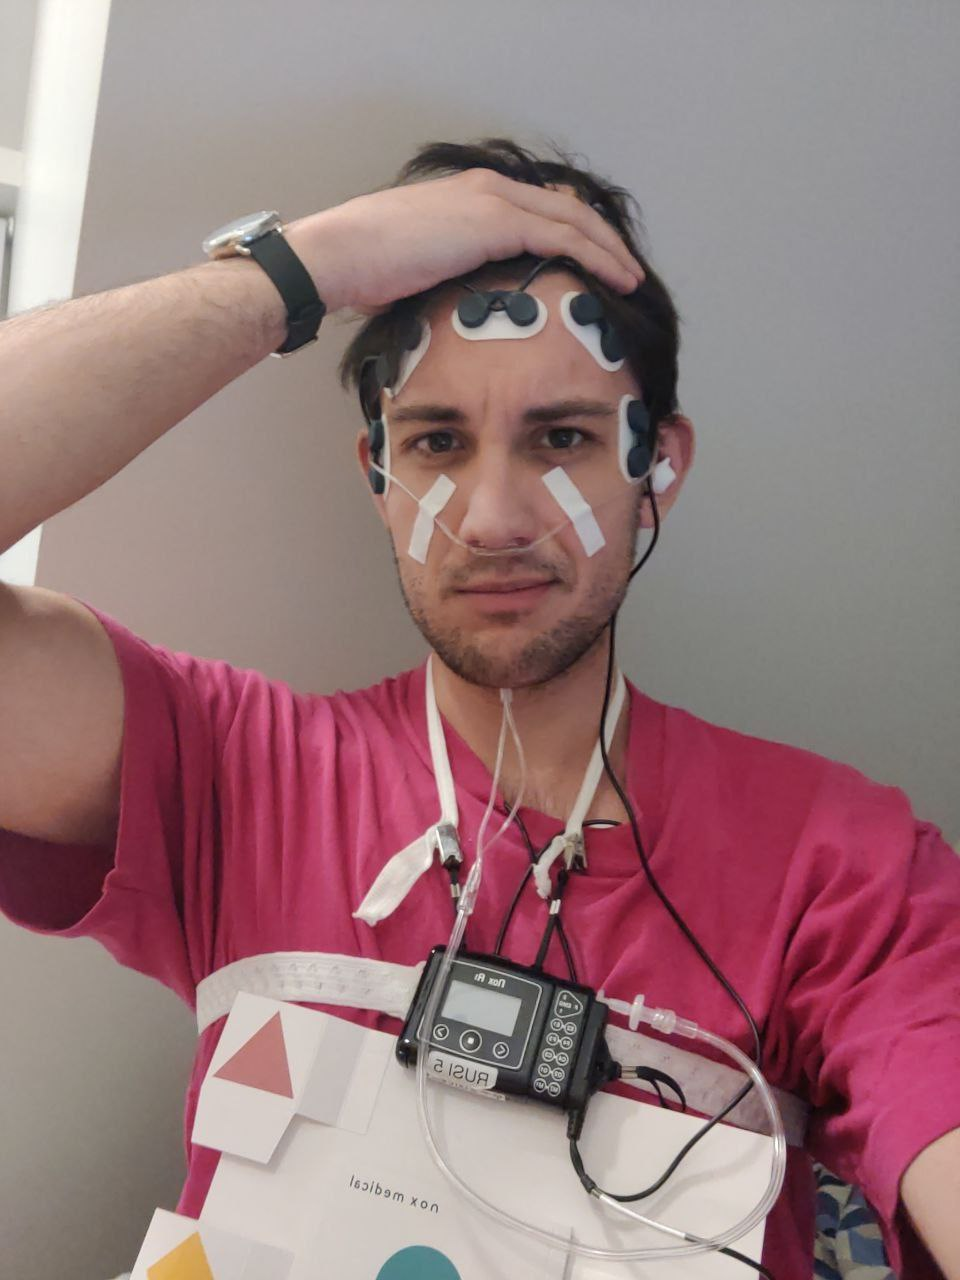
\includegraphics[width=0.2\linewidth]{imgs/martin-nox.png}
                    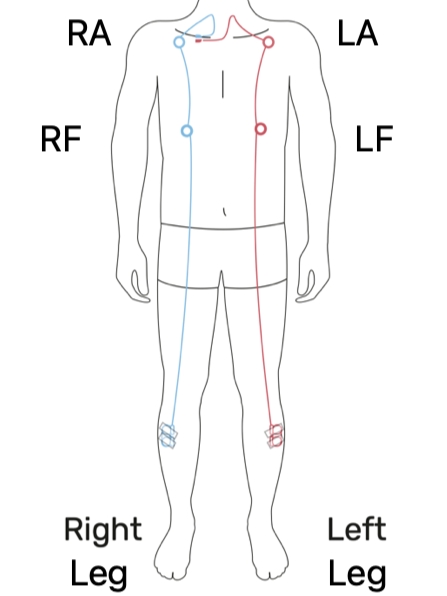
\includegraphics[width=0.2\linewidth]{imgs/electrodes_nox.png}
                    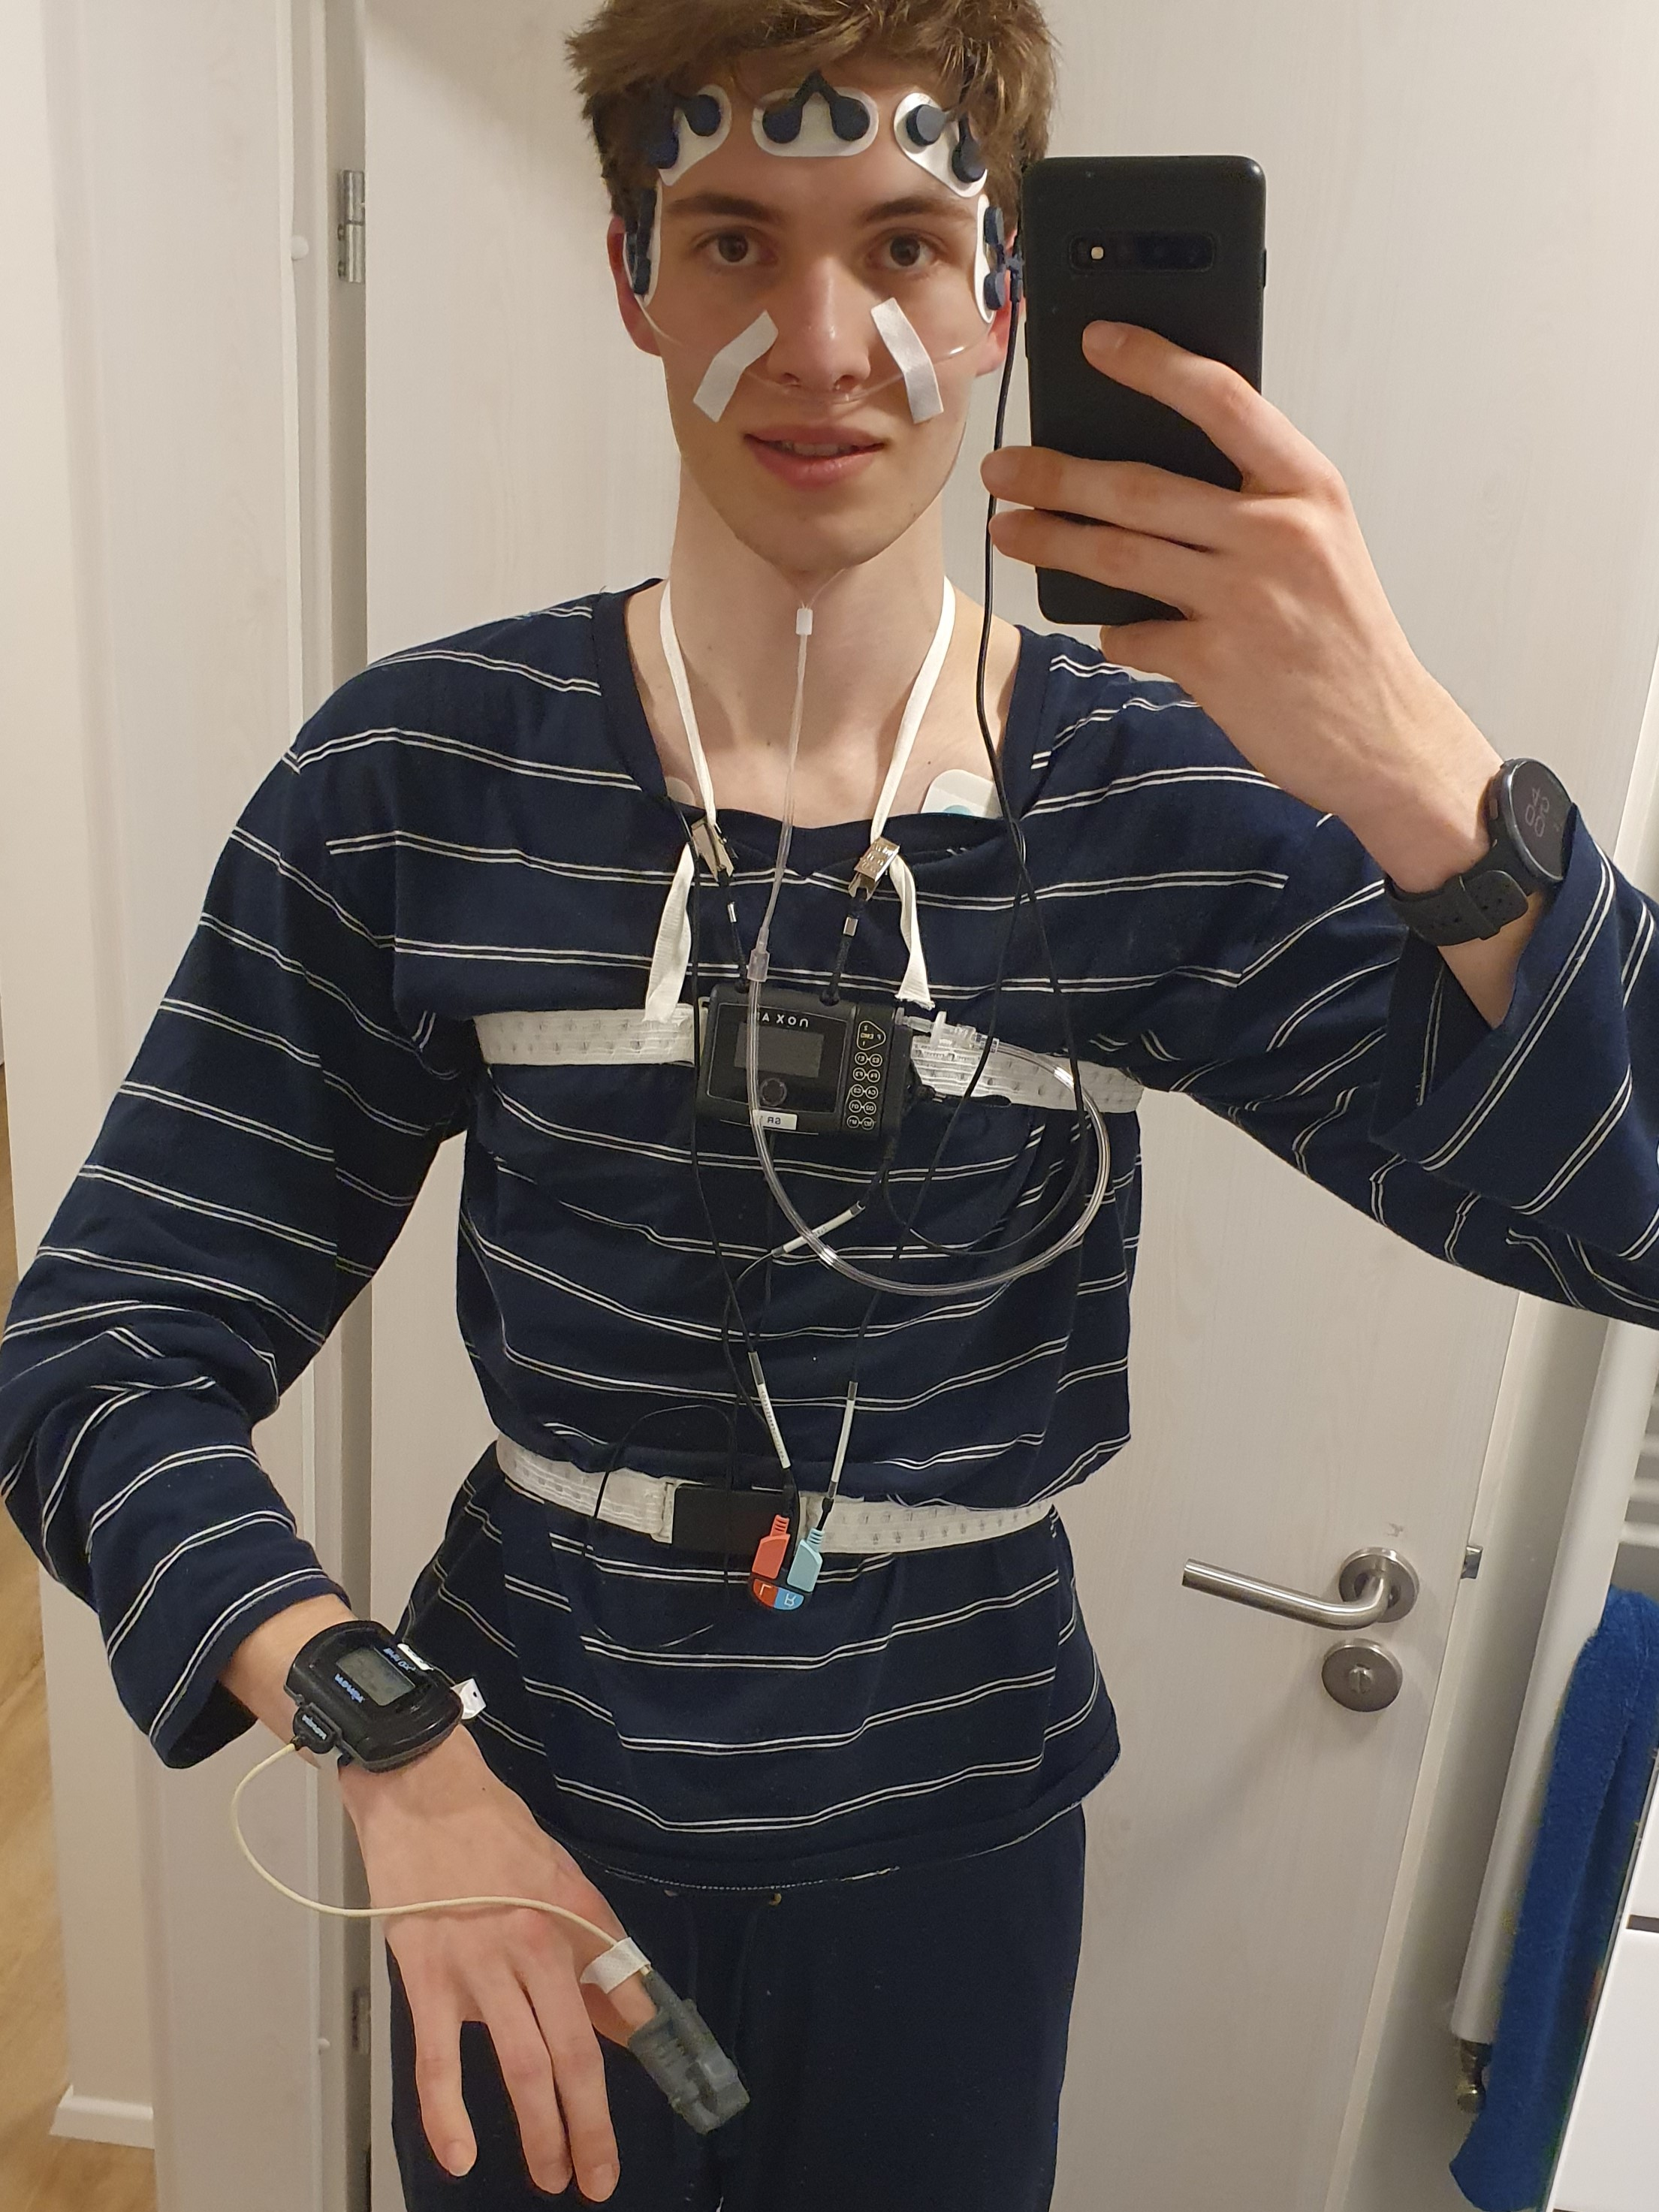
\includegraphics[width=0.2\linewidth]{imgs/nils_nox.jpg}
                    \caption{Setup of self-applied polysomnography}
                    \label{fig:setupPSG}
                \end{figure}
                \vspace{-0.7cm}
                \begin{columns}[t]
                    \begin{column}{0.45\linewidth}
                        \begin{itemize}
                            \item EEG, EOG and facial EMG from electrodes in the face
                            \item ECG and leg EMG from body cables
                        \end{itemize}
                    \end{column}

                    \hspace{-1.3cm}
                    
                    \begin{column}{0.55\linewidth}
                        \begin{itemize}
                            \item Thorax and abdomen belt, nasal pressure
                            \item Pulse oximeter for oxygen saturation
                            \item Audio and snoring signal, position, activity
                        \end{itemize}      
                    \end{column}
                \end{columns}
                % \begin{itemize}
                %     \item EEG, EOG and facial EMG from electrodes in the face
                %     \item ECG and leg EMG from body cables
                %     \item Thorax and abdomen belt, nasal pressure
                %     \item Pulse oximeter for oxygen saturation
                %     \item Audio and snoring signal, position, activity
                % \end{itemize}
            
            \end{block}

            \begin{block}{Difficulty of Sleep Scoring}
                Different sleep scorers may disagree when classifying certain sleep stages, particularly N1 and N3, as found in \cite{Rosenberg2013}. 
                This is also evident in Figure \autoref{fig:confidence-scorers}.

                \begin{figure}
                    \centering
                    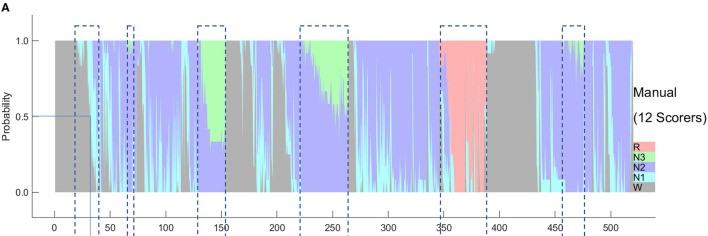
\includegraphics[width=0.9\linewidth]{imgs/confidence_scorers.jpg}
                    \caption{Confidence plot of scorings of 12 sleep scorers \cite{Anderer2023}}
                    \label{fig:confidence-scorers}
                \end{figure}
                \vspace{-0.5cm}
            \end{block}

            % \begin{block}{Sleep Staging with Smartwatches}
                
            %     \heading{Benefits}
            %     \begin{itemize}
            %         \item Objective measurement of sleep duration and continuity
            %         \item Easy to measure continuously for many days
            %         \item Non-intrusive assessment of "free living" sleep patterns
            %         \item Widespread consumer usage and accessibility
            %     \end{itemize}
                
            %     \heading{Limitations}
            %     \begin{itemize}
            %         \item Tend to overestimate sleep and underestimate wakefulness
            %         \item Cannot reliably differentiate sleep stages without proper physiological signals from the brain
            %         \item Very limited validation in clinical settings
            %         \item Often rely on black-box algorithms without transparent methodologies
            %     \end{itemize}
            %     \flushright{\small Source: Arnardóttir et al. 2021, Review}

            % \end{block}
	    
			\begin{block}{References}
				\printbibliography[heading=none]
			\end{block}
		\end{column}
		
		\separatorcolumn
	\end{columns}
\end{frame}
\end{document}
